\documentclass[conference]{IEEEtran}
\usepackage{booktabs,graphicx,url,xspace,amsmath}
\usepackage[hidelinks]{hyperref}
% AUTO-GENERATED by scripts/tables.py -- do not edit
\newcommand{\FCdxgenApk}{0.903}
\newcommand{\FCdxgenDeb}{0.828}
\newcommand{\FCdxgenMaven}{0.987}
\newcommand{\FCdxgenNodelock}{1.000}
\newcommand{\FCdxgenNodenolock}{1.000}
\newcommand{\FCdxgenNpm}{1.000}
\newcommand{\FCdxgenPyloose}{0.848}
\newcommand{\FCdxgenPypi}{0.928}
\newcommand{\FCdxgenPypinned}{1.000}
\newcommand{\FNCdxgenApk}{0}
\newcommand{\FNCdxgenDeb}{0}
\newcommand{\FNCdxgenMaven}{1}
\newcommand{\FNCdxgenNpm}{0}
\newcommand{\FNCdxgenPypi}{0}
\newcommand{\FNSyftApk}{0}
\newcommand{\FNSyftDeb}{0}
\newcommand{\FNSyftMaven}{2}
\newcommand{\FNSyftNpm}{0}
\newcommand{\FNSyftPypi}{0}
\newcommand{\FNTrivyApk}{0}
\newcommand{\FNTrivyDeb}{0}
\newcommand{\FNTrivyMaven}{0}
\newcommand{\FNTrivyNpm}{0}
\newcommand{\FNTrivyPypi}{0}
\newcommand{\FPCdxgenApk}{3}
\newcommand{\FPCdxgenDeb}{436}
\newcommand{\FPCdxgenMaven}{0}
\newcommand{\FPCdxgenNpm}{0}
\newcommand{\FPCdxgenPypi}{5}
\newcommand{\FPSyftApk}{0}
\newcommand{\FPSyftDeb}{0}
\newcommand{\FPSyftMaven}{4}
\newcommand{\FPSyftNpm}{0}
\newcommand{\FPSyftPypi}{0}
\newcommand{\FPTrivyApk}{0}
\newcommand{\FPTrivyDeb}{0}
\newcommand{\FPTrivyMaven}{0}
\newcommand{\FPTrivyNpm}{0}
\newcommand{\FPTrivyPypi}{0}
\newcommand{\FSyftApk}{1.000}
\newcommand{\FSyftDeb}{1.000}
\newcommand{\FSyftMaven}{0.923}
\newcommand{\FSyftNodelock}{1.000}
\newcommand{\FSyftNodenolock}{1.000}
\newcommand{\FSyftNpm}{1.000}
\newcommand{\FSyftPyloose}{1.000}
\newcommand{\FSyftPypi}{1.000}
\newcommand{\FSyftPypinned}{1.000}
\newcommand{\FTrivyApk}{1.000}
\newcommand{\FTrivyDeb}{1.000}
\newcommand{\FTrivyMaven}{1.000}
\newcommand{\FTrivyNodelock}{1.000}
\newcommand{\FTrivyNodenolock}{1.000}
\newcommand{\FTrivyNpm}{1.000}
\newcommand{\FTrivyPyloose}{1.000}
\newcommand{\FTrivyPypi}{1.000}
\newcommand{\FTrivyPypinned}{1.000}
\newcommand{\FailFEightCdxgen}{0}
\newcommand{\FailFEightSyft}{0}
\newcommand{\FailFEightTrivy}{0}
\newcommand{\FailFFiveCdxgen}{1}
\newcommand{\FailFFiveSyft}{2}
\newcommand{\FailFFiveTrivy}{0}
\newcommand{\FailFFourCdxgen}{0}
\newcommand{\FailFFourSyft}{2}
\newcommand{\FailFFourTrivy}{0}
\newcommand{\FailFOneCdxgen}{439}
\newcommand{\FailFOneSyft}{0}
\newcommand{\FailFOneTrivy}{0}
\newcommand{\FailFSevenCdxgen}{56}
\newcommand{\FailFSevenSyft}{132}
\newcommand{\FailFSevenTrivy}{117}
\newcommand{\FailFSixCdxgen}{0}
\newcommand{\FailFSixSyft}{18}
\newcommand{\FailFSixTrivy}{0}
\newcommand{\FailFThreeCdxgen}{0}
\newcommand{\FailFThreeSyft}{20}
\newcommand{\FailFThreeTrivy}{0}
\newcommand{\FailFTwoCdxgen}{5}
\newcommand{\FailFTwoSyft}{0}
\newcommand{\FailFTwoTrivy}{0}
\newcommand{\FailPOneCdxgen}{4}
\newcommand{\FailPOneSyft}{8}
\newcommand{\FailPOneTrivy}{0}
\newcommand{\JCdxgenSyft}{0.765}
\newcommand{\JCdxgenTrivy}{0.779}
\newcommand{\JMinCdxgenSyft}{0.630}
\newcommand{\JMinCdxgenTrivy}{0.692}
\newcommand{\JMinSyftTrivy}{0.814}
\newcommand{\JSyftTrivy}{0.978}
\newcommand{\JTomcatSyftTrivy}{0.814}
\newcommand{\NDetCases}{9}
\newcommand{\NDetIdentical}{9}
\newcommand{\NDetRuns}{4}
\newcommand{\NGTComponents}{1935}
\newcommand{\NImages}{12}
\newcommand{\NJarsNoMeta}{17}
\newcommand{\NNestedJars}{37}
\newcommand{\NSboms}{36}
\newcommand{\NSelfBuilt}{5}
\newcommand{\NValid}{36}
\newcommand{\OvAll}{1953}
\newcommand{\OvCdxOnly}{452}
\newcommand{\OvSyftOnly}{32}
\newcommand{\OvTrivyOnly}{0}
\newcommand{\OvUnion}{2458}
\newcommand{\PCdxgenApk}{0.824}
\newcommand{\PCdxgenDeb}{0.707}
\newcommand{\PCdxgenMaven}{1.000}
\newcommand{\PCdxgenNpm}{1.000}
\newcommand{\PCdxgenPypi}{0.865}
\newcommand{\PSyftApk}{1.000}
\newcommand{\PSyftDeb}{1.000}
\newcommand{\PSyftMaven}{0.900}
\newcommand{\PSyftNpm}{1.000}
\newcommand{\PSyftPypi}{1.000}
\newcommand{\PTrivyApk}{1.000}
\newcommand{\PTrivyDeb}{1.000}
\newcommand{\PTrivyMaven}{1.000}
\newcommand{\PTrivyNpm}{1.000}
\newcommand{\PTrivyPypi}{1.000}
\newcommand{\RCdxgenApk}{1.000}
\newcommand{\RCdxgenDeb}{1.000}
\newcommand{\RCdxgenMaven}{0.974}
\newcommand{\RCdxgenNpm}{1.000}
\newcommand{\RCdxgenPypi}{1.000}
\newcommand{\RSyftApk}{1.000}
\newcommand{\RSyftDeb}{1.000}
\newcommand{\RSyftMaven}{0.947}
\newcommand{\RSyftNpm}{1.000}
\newcommand{\RSyftPypi}{1.000}
\newcommand{\RTrivyApk}{1.000}
\newcommand{\RTrivyDeb}{1.000}
\newcommand{\RTrivyMaven}{1.000}
\newcommand{\RTrivyNpm}{1.000}
\newcommand{\RTrivyPypi}{1.000}
\newcommand{\RtMaxCdxgen}{24.7}
\newcommand{\RtMaxSyft}{5.2}
\newcommand{\RtMaxTrivy}{78.2}
\newcommand{\RtMedCdxgen}{11.7}
\newcommand{\RtMedSyft}{2.9}
\newcommand{\RtMedTrivy}{0.6}

\newcommand{\syft}{Syft\xspace}
\newcommand{\trivy}{Trivy\xspace}
\newcommand{\cdxgen}{cdxgen\xspace}
\newcommand{\RQ}[1]{\textbf{RQ#1}}

\begin{document}
\title{SBOM Generators Compared: Coverage and Accuracy of\\Syft, Trivy and cdxgen on Container Images}
\author{\IEEEauthorblockN{Yuvraj Deshmukh}
\IEEEauthorblockA{International Institute of Information Technology Bangalore\\
Supervisor: Prof.\ B.\ Thangaraju}}
\maketitle

\begin{abstract}
Software Bills of Materials (SBOMs) are becoming a regulatory and operational requirement, yet
different generators produce different component lists for the same artifact. We compare three widely
used open-source generators---\syft, \trivy and \cdxgen---on a corpus of \NImages{} \texttt{linux/amd64}
container images spanning Java, Node.js, Python and OS base images. For \NSelfBuilt{} self-built images
and for every queryable OS package database we extract ground truth from the installed artifacts
themselves (\NGTComponents{} components). All tools scan the same frozen image tarball; all
\NSboms{} CycloneDX SBOMs are schema-valid and every tool is deterministic across \NDetRuns{} runs.
\syft and \trivy reach perfect precision and recall on OS, npm and PyPI packages; \cdxgen also reaches
perfect recall but its OS-level precision drops to \PCdxgenDeb{} (Debian) because it additionally reports
source/origin packages as components, and it reports manifest version ranges from
\texttt{requirements.txt} as versions. Java fat jars are the hardest case: \NJarsNoMeta{} of
\NNestedJars{} nested jars carry no Maven metadata, which leads \syft to synthesize
\FailFThreeSyft{} incorrect Maven coordinates, whereas \trivy resolves them via a downloaded Java
database. Lock-file presence did not change accuracy for installed images. We release the full pipeline
and a practitioner decision table.
\end{abstract}

\begin{IEEEkeywords}
SBOM, software supply chain, CycloneDX, container security, DevSecOps, empirical study
\end{IEEEkeywords}

%=====================================================================
\section{Introduction}
An SBOM is a machine-readable inventory of the components contained in a software artifact. Since
U.S.\ Executive Order 14028~\cite{eo14028} and the EU Cyber Resilience Act~\cite{eucra}, SBOMs are moving
from good practice to obligation, and container images are one of the most common artifacts for which
they are produced. Every downstream use---vulnerability matching, licence compliance, incident
response---inherits the errors of the generator. Yet different tools report different component lists
for the same image, and their accuracy is rarely measured against ground truth.

We conduct a small but fully traceable comparative measurement study of three popular open-source
generators, \syft, \trivy and \cdxgen, and ask:
\begin{itemize}
\item \RQ1: Which tool finds the most real components per ecosystem (recall and precision)?
\item \RQ2: Where and why does each tool miss or mislabel components?
\item \RQ3: Does the presence of a lock file change tool accuracy?
\item \RQ4: How complete and consistent are version, PURL, licence and hash fields?
\end{itemize}
Our contributions are: (i) a ground-truth methodology for container images that derives truth from
installed artifacts rather than from package-manager manifests, including two pitfalls we encountered
(npm aliases, Spring Boot repackaging); (ii) a quantitative comparison with per-ecosystem
precision/recall and cross-tool overlap; (iii) a failure-pattern taxonomy with root causes; and (iv) a
reproducible pipeline in which every reported number is regenerated from saved raw outputs.

%=====================================================================
\section{Background}
\textbf{SBOM formats.} SPDX~\cite{spdx} (Linux Foundation, ISO/IEC 5962) originated in licence
compliance; CycloneDX~\cite{cyclonedx} (OWASP) originated in security use cases and is the native output
of all three tools studied. Both identify components primarily via Package URLs (PURLs)~\cite{purlspec},
e.g.\ \texttt{pkg:pypi/pyyaml@6.0.2} or \texttt{pkg:deb/debian/libc6@2.36-9}. We use CycloneDX JSON.

\textbf{Regulation.} EO~14028 led to NTIA's minimum elements for SBOMs (supplier, component name,
version, unique identifier, dependency relationship, author, timestamp). The EU CRA requires
manufacturers to draw up an SBOM covering at least top-level dependencies.

\textbf{Tools.} \syft (Anchore) and \trivy (Aqua Security) are Go binaries that catalogue OS package
databases and language-ecosystem metadata found in image layers; \trivy additionally resolves Java
archives via a downloaded SHA-1$\rightarrow$Maven-coordinate database. \cdxgen (OWASP CycloneDX) is a
Node.js tool covering many project types, including container images.

%=====================================================================
\section{Related Work}
Xia et al.~\cite{xia2023empirical} and Bi et al.~\cite{bi2023way} surveyed practitioners and SBOM
design issues, identifying tool immaturity as a key concern. Mirakhorli et al.~\cite{mirakhorli2024landscape}
mapped the landscape of open-source and proprietary SBOM tools. Balliu et al.~\cite{balliu2023java}
evaluated the accuracy of six SBOM producers on complex Java projects and reported hard challenges for
accurate production---consistent with our finding that Java archives are the main error source.
Halbritter and Merli~\cite{halbritter2024accuracy} evaluated SBOM tool accuracy for web applications and
system-level software. Wang et al.~\cite{wang2026adherence} studied the adherence of six tools to the SBOM
standards on 55,444 SBOMs from 3,287 repositories. Zhou et al.~\cite{zhou2025reality}, the closest
sibling study, analysed 2,414 repositories and showed that lock files with strong package managers enable
accurate and consistent SBOMs, while downstream scanners exhibited a 92.0\% false-positive rate.
O'Donoghue et al.~\cite{odonoghue2024impacts} examined how the choice of SBOM generator impacts vulnerability
detection. Novikov et al.~\cite{novikov2025policy} studied policy-driven SBOM adoption on GitHub.

For container scanners, Javed and Toor~\cite{javed2021container} and Kaur et al.~\cite{kaur2020container}
assessed vulnerability detection quality in images, and Churakova et al.~\cite{churakova2025vexed} used
Jaccard and Tversky indices to measure consistency among VEX tools on containers; we adopt Jaccard for
cross-tool agreement. Imtiaz et al.~\cite{imtiaz2021sca} provide the comparative design template we
follow. Unlike repository-level studies, we analyse built container images, where installed metadata
and manifests may disagree, and we derive ground truth from the installed artifacts.

%=====================================================================
\section{Methodology}
\subsection{Corpus}
Table~\ref{tab:corpus} lists the \NImages{} images. Five are self-built from small Dockerfiles so that
ground truth is fully known: a Spring Boot~3.3.5 uber-jar on \texttt{eclipse-temurin:21-jre}
(multi-stage, so the final image contains only the jar); two Node.js~22 apps with identical
dependencies, one installed via \texttt{npm ci} from a \texttt{package-lock.json} (with a
\texttt{devDependency}, \texttt{jest}, present in the lock but not installed) and one via
\texttt{npm install --no-package-lock} from caret ranges; and two Python~3.12 apps installed from a
pinned and a range-based (\texttt{django>=4.2,<5.0}) \texttt{requirements.txt}, which is left in the
image. The remaining seven are popular public images (Tomcat, Node, Python, Debian, Ubuntu, Alpine,
distroless). All images are pinned by digest and pulled/built for \texttt{linux/amd64} on an Apple
Silicon host (emulated).

\begin{table}[t]\centering\caption{Corpus (linux/amd64). Digest prefix shown; full digests in \texttt{results/corpus.csv}.}\label{tab:corpus}
\scriptsize\begin{tabular}{llllrl}\toprule
Image & Eco & Self & Lock & MB & Digest \\\midrule
sb-java-springboot & java & yes & no(fat-jar) & 114 & \texttt{104ffd6c9cb5} \\
tomcat & java & no & nan & 0 & \texttt{72cb796898f2} \\
sb-node-lock & node & yes & yes & 75 & \texttt{8e1c73c3e3db} \\
sb-node-nolock & node & yes & no & 75 & \texttt{d2728c34b2b6} \\
node & node & no & nan & 0 & \texttt{f035ba7ffee1} \\
sb-py-pinned & python & yes & yes(pinned) & 69 & \texttt{1395364c8b05} \\
sb-py-loose & python & yes & no(ranges) & 76 & \texttt{8e7fd34ff1d5} \\
python & python & no & nan & 0 & \texttt{60d9996b6a8a} \\
debian & os & no & nan & 0 & \texttt{36e591f228bb} \\
ubuntu & os & no & nan & 0 & \texttt{68ee22004a91} \\
alpine & os & no & nan & 0 & \texttt{1e42bbe25081} \\
distroless & os & no & nan & 0 & \texttt{fabbf1c0c357} \\
\bottomrule\end{tabular}\end{table}


\subsection{Ground truth}
Ground truth is extracted from inside each image: \texttt{dpkg-query} (status \texttt{ii} only) or
\texttt{apk info -v} for OS packages; distroless's \texttt{/var/lib/dpkg/status.d}; \texttt{pip list}
for Python. We found two cases where package-manager listings do \emph{not} reflect installed reality
and therefore switched to artifact-level truth:
\begin{itemize}
\item \textbf{npm aliases.} \texttt{npm ls} reports aliased dependencies under their alias
(e.g.\ \texttt{string-width-cjs}), whereas the installed \texttt{package.json} declares
\texttt{string-width}. We walk every \texttt{node\_modules} tree (app, global, \texttt{/opt/yarn*}) and
read each \texttt{package.json}; this also surfaced \texttt{yarn}~1.22.22, shipped in the Node base
image outside npm's global tree.
\item \textbf{Spring Boot repackaging.} \texttt{mvn dependency:list} includes the
\texttt{spring-boot-starter-*} artifacts, which are not present in \texttt{BOOT-INF/lib} of the built jar, and omits \texttt{spring-boot-jarmode-tools}, which the repackager
injects. Truth is therefore the set of jars physically in \texttt{BOOT-INF/lib}
(\NNestedJars{} jars), with coordinates resolved from the build's resolved dependency list.
\end{itemize}
The application itself (e.g.\ \texttt{edu.iiitb.sbom:demo}) is counted as a true component. For public
images only the OS layer (and Python/npm runtimes where queryable) has ground truth; Tomcat's jars have
none and are evaluated only by cross-tool agreement.

\subsection{SBOM generation}
Each image is exported once with \texttt{docker save --platform linux/amd64} and all three tools scan the
identical tarball (\syft: \texttt{docker-archive:}; \trivy: \texttt{image --input}; \cdxgen:
\texttt{-t docker}). This removes registry/daemon differences and was necessary because the Docker
daemon's containerd store could not export multi-architecture images to \trivy/\cdxgen. Tools run with
default settings except \cdxgen's \texttt{--spec-version 1.6}. Versions: \syft~1.55.0, \trivy~0.76.1,
\cdxgen~12.9.0, CycloneDX CLI~0.33.1. Each run's wall-clock time and exit code is logged. Three images
were scanned \NDetRuns{} times per tool to test determinism. Every SBOM was validated with
\texttt{cyclonedx validate} against its declared spec version.

\subsection{Normalisation and metrics}
Each component is mapped to a key (ecosystem, name, version) from its PURL: PyPI names are normalised
per PEP~503; Maven names are \texttt{group:artifact}; npm names include the scope; OS distro namespaces
and qualifiers are dropped and Debian epochs stripped (tools disagree on epoch placement). Components of
type \texttt{file}, \texttt{operating-system}, \texttt{cryptographic-asset} and \texttt{data} are
excluded. Against ground truth we compute precision, recall and F1 per image and pooled (micro-average)
per component ecosystem, at name and name+version level. Only ecosystems covered by an image's ground
truth are scored; components in other ecosystems are reported separately and never counted as false
positives. Across all images we compute pairwise Jaccard similarity and exclusive overlap regions, and
field completeness per tool.

%=====================================================================
\section{Results}
\subsection{RQ1: Coverage and accuracy}
Table~\ref{tab:byeco} and Fig.~\ref{fig:eco} report pooled results. All three tools achieve recall
$1.000$ on Debian, Alpine, npm and PyPI packages: no installed OS or Python/Node package was missed by
any tool. Differences lie in precision and in Java.
\syft and \trivy have precision $1.000$ on all non-Java ecosystems. \cdxgen's precision is
\PCdxgenDeb{} on Debian (\FPCdxgenDeb{} extra entries), \PCdxgenApk{} on Alpine and \PCdxgenPypi{} on PyPI.
On the Spring Boot fat jar, \trivy is exact (F1 \FTrivyMaven), \cdxgen misses one jar
(F1 \FCdxgenMaven), and \syft has F1 \FSyftMaven{} (\FPSyftMaven{} false positives, \FNSyftMaven{} misses).
Fig.~\ref{fig:heat} shows per-image F1; Table~\ref{tab:perimage} splits OS and language layers.

\begin{table*}[t]\centering\caption{Precision / recall / F1 against ground truth, pooled over all images with ground truth, matched on (ecosystem, name, version). $|GT|$ = number of ground-truth components.}\label{tab:byeco}
\small\begin{tabular}{lr ccc ccc ccc}\toprule
 & & \multicolumn{3}{c}{Syft} & \multicolumn{3}{c}{Trivy} & \multicolumn{3}{c}{cdxgen}\\
\cmidrule(lr){3-5}\cmidrule(lr){6-8}\cmidrule(lr){9-11}
Eco & $|GT|$ & P & R & F1 & P & R & F1 & P & R & F1 \\\midrule
deb & 1053 & 1.000 & 1.000 & 1.000 & 1.000 & 1.000 & 1.000 & 0.707 & 1.000 & 0.828 \\
apk & 14 & 1.000 & 1.000 & 1.000 & 1.000 & 1.000 & 1.000 & 0.824 & 1.000 & 0.903 \\
pypi & 32 & 1.000 & 1.000 & 1.000 & 1.000 & 1.000 & 1.000 & 0.865 & 1.000 & 0.928 \\
npm & 798 & 1.000 & 1.000 & 1.000 & 1.000 & 1.000 & 1.000 & 1.000 & 1.000 & 1.000 \\
maven & 38 & 0.900 & 0.947 & 0.923 & 1.000 & 1.000 & 1.000 & 1.000 & 0.974 & 0.987 \\
\bottomrule\end{tabular}\end{table*}


\begin{figure}[t]\centering
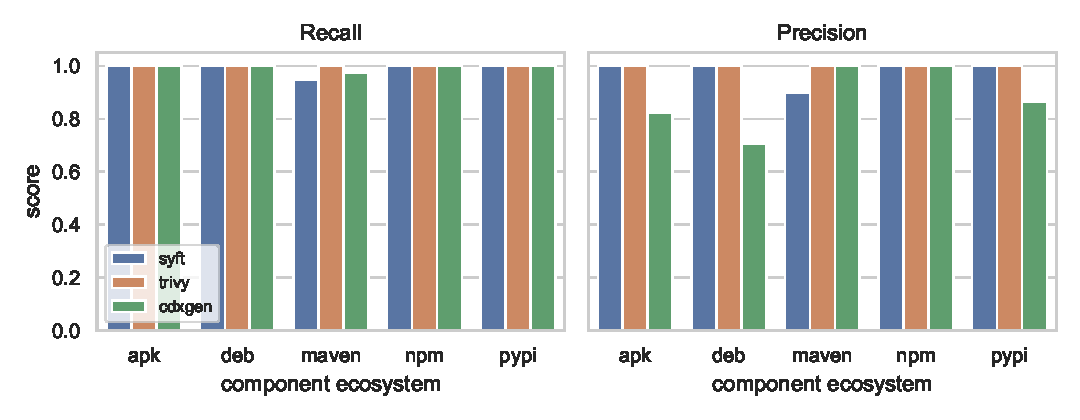
\includegraphics[width=\columnwidth]{../figures/fig1_recall_precision_by_eco.pdf}
\caption{Pooled recall and precision per component ecosystem (name+version).}\label{fig:eco}
\end{figure}

\textbf{Cross-tool agreement.} Mean pairwise Jaccard over all \NImages{} images is \JSyftTrivy{}
(\syft--\trivy), \JCdxgenSyft{} (\cdxgen--\syft) and \JCdxgenTrivy{} (\cdxgen--\trivy). Of
\OvUnion{} distinct (image, ecosystem, name, version) keys, \OvAll{} are reported by all three tools,
\OvCdxOnly{} only by \cdxgen, \OvSyftOnly{} only by \syft and \OvTrivyOnly{} only by \trivy
(Fig.~\ref{fig:upset}). On Tomcat, where no Java ground truth exists, \syft--\trivy agreement drops to
\JTomcatSyftTrivy{}, driven by Java coordinates (Section~\ref{sec:fail}).

\begin{figure}[t]\centering
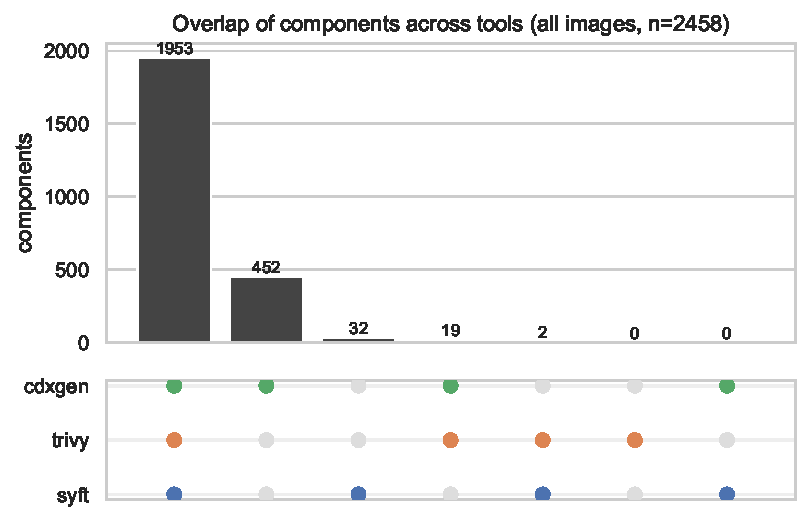
\includegraphics[width=\columnwidth]{../figures/fig2_upset_overlap.pdf}
\caption{Exclusive overlap of component keys across tools, all images.}\label{fig:upset}
\end{figure}

\begin{figure}[t]\centering
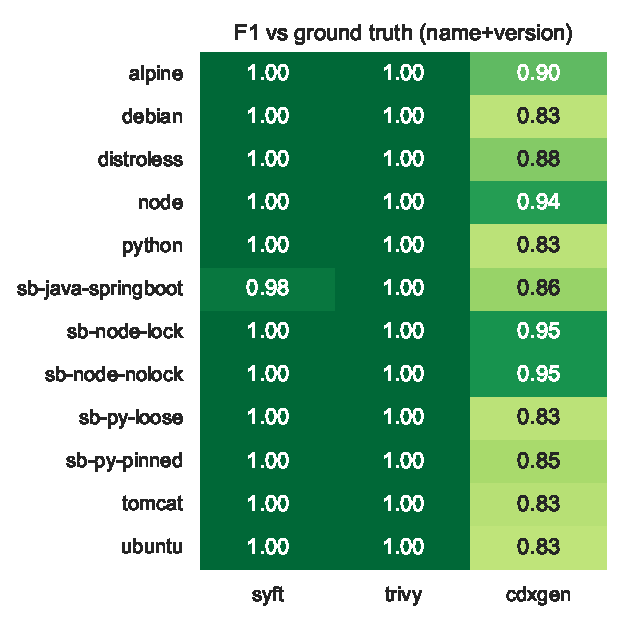
\includegraphics[width=0.85\columnwidth]{../figures/fig3_f1_heatmap.pdf}
\caption{Per-image F1 against ground truth (scored ecosystems only).}\label{fig:heat}
\end{figure}

\begin{table}[t]\centering\caption{Per-image F1 (name+version) by layer: OS packages vs.\ language packages.}\label{tab:perimage}
\scriptsize\begin{tabular}{llccc}\toprule
Image & Layer & Syft & Trivy & cdxgen \\\midrule
alpine & os & 1.000 & 1.000 & 0.903 \\
debian & os & 1.000 & 1.000 & 0.826 \\
distroless & os & 1.000 & 1.000 & 0.875 \\
node & lang & 1.000 & 1.000 & 1.000 \\
node & os & 1.000 & 1.000 & 0.826 \\
python & lang & 1.000 & 1.000 & 1.000 \\
python & os & 1.000 & 1.000 & 0.827 \\
sb-java-springboot & lang & 0.923 & 1.000 & 0.987 \\
sb-java-springboot & os & 1.000 & 1.000 & 0.834 \\
sb-node-lock & lang & 1.000 & 1.000 & 1.000 \\
sb-node-lock & os & 1.000 & 1.000 & 0.826 \\
sb-node-nolock & lang & 1.000 & 1.000 & 1.000 \\
sb-node-nolock & os & 1.000 & 1.000 & 0.826 \\
sb-py-loose & lang & 1.000 & 1.000 & 0.848 \\
sb-py-loose & os & 1.000 & 1.000 & 0.827 \\
sb-py-pinned & lang & 1.000 & 1.000 & 1.000 \\
sb-py-pinned & os & 1.000 & 1.000 & 0.827 \\
tomcat & os & 1.000 & 1.000 & 0.832 \\
ubuntu & os & 1.000 & 1.000 & 0.825 \\
\bottomrule\end{tabular}\end{table}


\textbf{Operational properties.} All \NSboms{} SBOMs were schema-valid (\NValid/\NSboms).
All \NDetCases{} tool$\times$image determinism cases produced identical component sets in
\NDetRuns{} runs (\NDetIdentical/\NDetCases). Median scan time per image was \RtMedTrivy\,s (\trivy),
\RtMedSyft\,s (\syft) and \RtMedCdxgen\,s (\cdxgen); \trivy's maximum (\RtMaxTrivy\,s) is a one-off
download of its Java database on the first jar scan.

\subsection{RQ3: Lock files}
On the Node pair, all three tools achieve identical language-layer F1 with and without a lock file
(\syft \FSyftNodelock/\FSyftNodenolock, \trivy \FTrivyNodelock/\FTrivyNodenolock,
\cdxgen \FCdxgenNodelock/\FCdxgenNodenolock): in built images the tools read installed
\texttt{node\_modules} metadata, so the lock file adds no information, and none reported the
uninstalled \texttt{devDependency}. On the Python pair, \syft and \trivy are unaffected
(\FSyftPypinned/\FSyftPyloose, \FTrivyPypinned/\FTrivyPyloose), whereas \cdxgen drops from
\FCdxgenPypinned{} to \FCdxgenPyloose{} because it also emits the lower bound of each range in
\texttt{requirements.txt} as a version (pattern F2). Thus, unlike repository-level
scanning~\cite{zhou2025reality}, lock files matter little once dependencies are installed---unless a
tool mixes manifest parsing with installed-metadata cataloguing.

\subsection{RQ4: Field completeness}
Table~\ref{tab:fields} summarises fields. All tools emit valid PURLs and versions for nearly all
components. Licence coverage is high for \syft and \trivy across ecosystems; \cdxgen reports licences
for npm but rarely for OS packages or Maven. Hashes differ by design: \trivy emits hashes for language
packages, \cdxgen for many OS packages, \syft for none in CycloneDX output. Only \syft emits CPEs.

\begin{table}[t]\centering\caption{Field completeness (\% of component entries). os = deb+apk.}\label{tab:fields}
\scriptsize\setlength{\tabcolsep}{3pt}\begin{tabular}{llrrrrrrr}\toprule
Tool & Eco & $n$ & PURL & Ver & Lic & Hash & Supp & CPE \\\midrule
Syft & maven & 82 & 100 & 100 & 92 & 0 & 0 & 100 \\
Syft & npm & 915 & 100 & 100 & 100 & 0 & 95 & 100 \\
Syft & os & 1067 & 100 & 100 & 100 & 0 & 100 & 100 \\
Syft & pypi & 32 & 100 & 100 & 94 & 0 & 81 & 100 \\
Trivy & maven & 77 & 100 & 100 & 94 & 100 & 0 & 0 \\
Trivy & npm & 915 & 100 & 100 & 100 & 100 & 0 & 0 \\
Trivy & os & 1067 & 100 & 100 & 94 & 12 & 100 & 0 \\
Trivy & pypi & 32 & 100 & 100 & 100 & 100 & 0 & 0 \\
cdxgen & maven & 75 & 100 & 100 & 4 & 4 & 0 & 0 \\
cdxgen & npm & 800 & 100 & 100 & 99 & 0 & 0 & 0 \\
cdxgen & os & 1562 & 100 & 100 & 1 & 69 & 100 & 0 \\
cdxgen & pypi & 37 & 100 & 97 & 62 & 0 & 27 & 0 \\
\bottomrule\end{tabular}\end{table}


%=====================================================================
\section{Failure Patterns (RQ2)}\label{sec:fail}
We inspected every disagreement against ground truth and the Tomcat cross-tool disagreements, and
quantify each pattern programmatically (Table~\ref{tab:failures}).

\textbf{F1: OS source/origin packages (\cdxgen, \FailFOneCdxgen{} entries).} For Debian, \cdxgen emits
an extra \texttt{library} component for each \emph{source} package (e.g.\ \texttt{acl}, \texttt{attr},
\texttt{bzip2}, \texttt{glibc}) in addition to the installed binary packages; for Alpine it emits
\emph{origin} packages (\texttt{openssl} for \texttt{libssl3}/\texttt{libcrypto3}). These entries carry
no property distinguishing them from installed packages, so consumers cannot filter them. This alone
explains \cdxgen's OS precision.

\textbf{F2: Manifest ranges as versions (\cdxgen, \FailFTwoCdxgen).} With range-based
\texttt{requirements.txt}, \cdxgen reports e.g.\ \texttt{pyyaml@5.1} (from \texttt{>=5.1}) and an
unversioned \texttt{numpy} next to the installed versions---the naive requirements parsing also noted
in industry reports.

\textbf{F3: Synthesised Maven coordinates (\syft, \FailFThreeSyft).} \NJarsNoMeta{} of the
\NNestedJars{} nested jars (including all Spring Framework and embedded Tomcat jars) lack
\texttt{META-INF/maven/.../pom.properties}. \syft then derives coordinates from manifest fields,
producing \texttt{checker-qual:checker-qual} instead of \texttt{org.checkerframework:checker-qual},
\texttt{org.apache.tomcat-catalina:catalina}, a Java class name used as group
(\texttt{org.springframework.boot.loader.launch.JarLauncher}), and on Tomcat specification versions
(\texttt{servlet-api@6.0}) rather than implementation versions (\texttt{tomcat-servlet-api@10.1.31}).
\trivy avoids this by looking up jar SHA-1 digests in its Java DB.

\textbf{F4: JDK internals (\syft, \FailFFourSyft).} \syft reports the JDK's
\texttt{lib/jrt-fs.jar} as a Maven package. \textbf{F5: missed nested jars} (\syft \FailFFiveSyft,
\cdxgen \FailFFiveCdxgen), e.g.\ \cdxgen omits \texttt{tomcat-embed-websocket}; \syft's two misses are
the correctly-named counterparts of its F3 mislabels.
\textbf{F6: non-package artifacts (\syft, \FailFSixSyft).} \syft reports Windows launcher executables
bundled in pip's \texttt{distlib} as PURL-less ``Simple Launcher'' components.
\textbf{F7: duplicates} are mostly legitimate (the same npm package installed at several paths), but
\cdxgen also duplicates Debian packages across architectures.
\textbf{F8: dev dependencies}: no tool reported the uninstalled \texttt{jest} (0 for all).
Conversely, \syft (\FailPOneSyft) and \cdxgen (\FailPOneCdxgen) detect language runtime binaries
(\texttt{node}, \texttt{python}, \texttt{openjdk}) that are not registered with any package manager---a
coverage advantage our ground truth does not credit.

\begin{table}[t]\centering\caption{Failure patterns $\times$ tool (counts of affected component entries, all images). P1 is a capability beyond the ground truth, not a failure.}\label{tab:failures}
\scriptsize\begin{tabular}{p{4.6cm}rrr}\toprule
Pattern & Syft & Trivy & cdxgen \\\midrule
OS source/origin package reported as installed package & 0 & 0 & 439 \\
manifest version range reported as version (requirements.txt) & 0 & 0 & 5 \\
synthesized/incorrect Maven groupId (jar lacks pom.properties) & 20 & 0 & 0 \\
JDK-internal jar reported as Maven package (jrt-fs) & 2 & 0 & 0 \\
nested jar inside fat jar missed & 2 & 0 & 1 \\
non-package artifact without PURL (e.g. bundled .exe launchers) & 18 & 0 & 0 \\
duplicate (eco,name,version) entries (mostly legitimate multiple install paths) & 132 & 117 & 56 \\
devDependency (in lock, not installed) reported & 0 & 0 & 0 \\
language runtime binary detected (node/python/openjdk) [beyond GT] & 8 & 0 & 4 \\
\bottomrule\end{tabular}\end{table}


%=====================================================================
\section{Discussion and Practitioner Guidance}
For OS packages and installed npm/PyPI dependencies, \syft and \trivy are interchangeable and exact on
our corpus; tool choice matters primarily for (a) Java archives, where identification without embedded
metadata requires a hash database (\trivy) or produces guessed coordinates (\syft), and (b) \cdxgen's
inclusion of source/origin packages and manifest ranges, which inflates component counts and will
produce spurious vulnerability matches downstream. Because no tool dominates every dimension
(\syft: CPEs, runtime binaries, licences; \trivy: Java accuracy, hashes; \cdxgen: OS hashes),
organisations that rely on SBOMs for compliance should pin a tool version, record its databases, and
spot-check against installed metadata. A one-page decision table accompanies this paper
(\texttt{paper/practitioner\_guide.md}).

%=====================================================================
\section{Threats to Validity}
\textbf{Construct.} Ground truth is limited to package-manager-registered components plus the jars in
the fat jar; statically linked binaries, vendored code and runtimes are not counted, so tools that find
them (P1) are not credited and their precision on such items is unmeasured. We corrected two
ground-truth extraction pitfalls (npm aliases, Spring Boot repackaging); further unknown pitfalls may
exist. Normalisation decisions (epoch stripping, PEP~503) affect matching.
\textbf{Internal.} \trivy's Java results depend on a network-fetched Java DB (recorded in
\texttt{versions.md}); results may change as the DB updates. All scans ran under amd64 emulation on an
arm64 host; outputs were deterministic, but runtimes are not representative of native performance.
\textbf{External.} The corpus is small (\NImages{} images, one Java fat jar with ground truth, no Go/Rust/
.NET), single-platform and uses default tool settings; results may not generalise. We evaluated
CycloneDX output only.
\textbf{Tool versions and supply chain.} Results hold for the pinned versions only. \trivy itself suffered
a supply-chain compromise in March 2026 (GHSA-69fq-xp46-6x23 / CVE-2026-33634; malicious v0.69.4
binaries, v0.69.5--0.69.6 images and GitHub Action tags)~\cite{trivyadvisory}; we used v0.76.1, outside
the affected range, illustrating that SBOM tooling is itself part of the supply chain.

%=====================================================================
\section{Conclusion}
On \NImages{} container images, \syft and \trivy produced exact SBOMs for OS, npm and PyPI packages,
while \cdxgen matched their recall but added source/origin packages and manifest ranges that reduce
precision. Java fat jars remain the main source of error, chiefly because many jars carry no Maven
metadata. Lock files had no effect on installed images. Future work: larger and multi-platform corpora,
Go/Rust binaries, SPDX output, and the downstream effect of these errors on vulnerability matching.

\section*{Reproducibility}
All scripts, raw SBOMs, ground-truth extracts, and the generator for every table and number in this
paper (\texttt{scripts/tables.py}) are in the project repository; \texttt{make all} regenerates them.

\bibliographystyle{IEEEtran}
\bibliography{refs}
\end{document}
